\documentclass[a4paper, 14pt]{extarticle}%тип документа

%Русский язык
\usepackage[T2A]{fontenc} %кодировка
\usepackage[utf8]{inputenc} %кодировка исходного кода
\usepackage[english,russian]{babel} %локализация и переносы

%отступы 
\usepackage[left=2cm,right=2cm,top=2cm,bottom=3cm,bindingoffset=0cm]{geometry}

%Вставка картинок
\usepackage{graphicx}
\usepackage{wrapfig, caption}
\graphicspath{}
\DeclareGraphicsExtensions{.pdf,.png,.jpg, .jpeg}
\newcommand\ECaption[1]{%
     \captionsetup{font=footnotesize}%
     \caption{#1}}

%Таблицы
\usepackage[table,xcdraw]{xcolor}
\usepackage{booktabs}

%Графики
\usepackage{pgfplots}
\pgfplotsset{compat=1.9}

%Математика
\usepackage{amsmath, amsfonts, amssymb, amsthm, mathtools}

%Заголовок
\author{Подлесный Артём \\ группа 827}
\title{Работа 3.3.4 \\ Эффект Холла в полупроводниках}

\begin{document}
\maketitle
\paragraph*{Цель работы:}
измерение подвижности и концентрации носителей заряда в полупроводниках.
\paragraph*{Оборудование:}
электромагнит с источником питания GPR, батарейка 1.5 В, амперметр, реостат, цифровой вольтметр, милливеббеметр, образцы легированного германия.
\section*{Общая теория}
\subsection*{Зонная модель}
Соударения электронов с решеткой можно рассматривать как вязкое трение, поэтому для средней скорости упорядоченного движения получаем:
\[\langle\vec{v}\rangle = -b\vec{E},\]
где $b$ - подвижность. Получаем силу действия кристаллической решетки на электроны:
\[\vec{F_{\text{тр}}} = -\frac{e}{b}\langle\vec{v}\rangle.\]
Если концентрация электронов равна $n$, то плотность тока будет определяться простым соотношением:
\[j = en\langle v\rangle=enbE.\]
Таким образом получаем закон Ома:
\begin{equation}
j = \sigma E \text{, где } \sigma=enb.
\end{equation}
Здесь $\sigma$ -- это электрическая проводимость. Для полупроводников в общем случае, когда в процессе проводимости участвуют и электроны, и дырки, проводимость определяется таким соотношением:
\[\sigma = e(nb_{\varepsilon}+pb_p),\]
где $n$, и $p$ -- концентрации электронов и дырок, $b$ -- их проводимости.
\subsection*{Эффект Холла в металлах и полупроводниках}
Суть эффекта Холла состоит в следующем. Пусть через однородную пластину металла вдоль оси $x$ течет ток $I$ (рис 1).

\begin{wrapfigure}{l}{0.3\textwidth}
\begin{center}
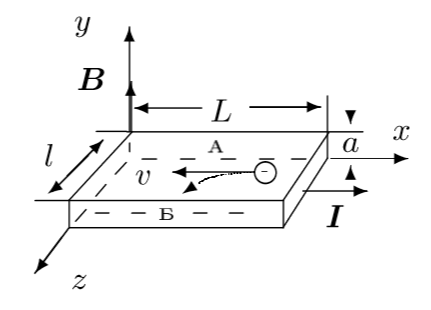
\includegraphics[height=3cm]{teor.png}
\end{center}
\ECaption{Образец с током в магнитном поле.}
\end{wrapfigure}

Если этот образец поместить в магнитное поле, направленное по оси $y$, то между пластинами А и Б возникнет разность потенциалов, и на электрон будет действовать сила Лоренца:
\begin{equation}
\vec{F_{\text{л}}} = -e\vec{E} - e\langle\vec{v}\rangle\times\vec{B}.
\end{equation}
В нашем случае сила, обусловленная вторым слагаемым направлена вдоль оси $z$ и равна
\[F_B = e\vert\langle v_x\rangle\vert B.\]
Здесь $\langle v_x\rangle$ -- это абсолютная величина дрейфовой скорости электронов. Из условие равновесия $F_B = F_E$ находим:
\[E_z = \vert\langle v_x\rangle\vert B.\]
С полем $E_z$ связана разность потенциалов между пластинами А и Б:
\[U_{\text{АБ}} = -E_zl= -\vert\langle v_x\rangle\vert Bl\]
В этом и состоит эффект Холла. Тк сила тока 
\[I = ne\vert\langle v_x\rangle\vert l\cdot a,\]
то находим ЭДС Холла:
\begin{equation}
\xi_x = U_{\text{АБ}} = -\frac{IB}{nea}=-R_x\cdot\frac{IB}{a}.
\end{equation}
Константа $R_x$ называется постоянной Холла. Она равна, как видно,
\begin{equation}
R_x = \frac{1}{ne}.
\end{equation}
В полупроводниках выражение для постоянной Холла более сложное:
\[R_x = \dfrac{nb_e^2 - pb_p^2}{e(nb_e+pb_p)^2}.\]
\section*{Экспериментальная установка}
\begin{figure}[h!]
\begin{center}
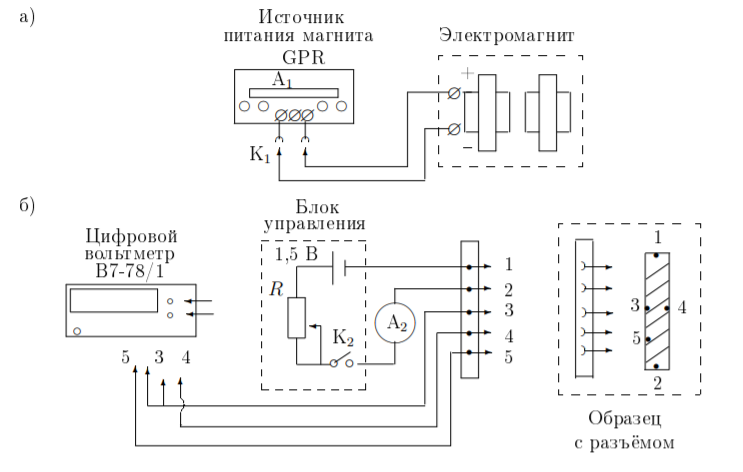
\includegraphics[width=0.9\textwidth]{ust}
\end{center}
\ECaption{Экспериментальная установка}
\end{figure}
Рассчитать проводимость образца можно, зная параметры установки, по следующей формуле:
\begin{equation}
\sigma=\dfrac{IL_{35}}{U_{35}al}
\end{equation}
\section*{Экспериментальные данные}
\subsection*{Градуировка электромагнита}
Была исследована зависимость потока электромагнитной индукции в зазоре электромагнита $\Phi$ от тока $I_M$ через его  обмотки. Она представлена на таблице.

\begin{table}[h!]
\begin{center}
\begin{tabular}{|l|l|l|}
\hline
\rowcolor[HTML]{FFFFC7} 
$I$, A & Ф, мВб & $B$, мТл \\ \hline
0.2    & 1.4    & 194.44   \\ \hline
\rowcolor[HTML]{FFFFC7} 
0.4    & 2.7    & 375.00   \\ \hline
0.6    & 4      & 555.56   \\ \hline
\rowcolor[HTML]{FFFFC7} 
0.8    & 5.2    & 722.22   \\ \hline
1      & 6.3    & 875.00   \\ \hline
\rowcolor[HTML]{FFFFC7} 
1.2    & 7.1    & 986.11   \\ \hline
1.4    & 7.7    & 1069.44  \\ \hline
\rowcolor[HTML]{FFFFC7} 
1.58   & 8      & 1111.11  \\ \hline
\end{tabular}
\end{center}
\ECaption{Градуировка электромагнита}
\end{table}
\subsection*{Измерение ЭДС Холла}
Измерения проводились в соответствии с методичкой, начальное напряжение на вольтметре - $U_0$. В зависимости от тока на обмотке магнита $I_M$, и, в более общем случае, от тока через образец $I$, измерялось напряжение на выходах 3-4 образца, которое и было ЭДС Холла. Все измерения представлены на "очень большой таблице".
\begin{table}[h!]
\begin{tabular}{|c|c|c|c|c|c|c|c|c|c|c|}
\hline
\rowcolor[HTML]{FFFFC7} 
$I$, мА : & $U_0$, мкВ : & $U_0+U_{34}$, мкВ & 30  & 56  & 75  & 96  & 115 & 127 & 135 & 142  \\ \hline
0.3       & 9            & $I_M$, мА          & 0.2 & 0.4 & 0.6 & 0.8 & 1   & 1.2 & 1.4 & 1.59 \\ \hline
\rowcolor[HTML]{FFFFC7} 
0.4       & 23           & $U_0+U_{34}$, мкВ & 54  & 85  & 114 & 140 & 165 & 182 & 195 & 202  \\ \hline
          &              & $I_M$, мА          & 0.2 & 0.4 & 0.6 & 0.8 & 1   & 1.2 & 1.4 & 1.59 \\ \hline
\rowcolor[HTML]{FFFFC7} 
0.5       & 28           & $U_0+U_{34}$, мкВ & 65  & 102 & 141 & 175 & 206 & 229 & 241 & 252  \\ \hline
          &              & $I_M$, мА          & 0.2 & 0.4 & 0.6 & 0.8 & 1   & 1.2 & 1.4 & 1.59 \\ \hline
\rowcolor[HTML]{FFFFC7} 
0.6       & 33           & $U_0+U_{34}$, мкВ & 78  & 125 & 170 & 212 & 248 & 273 & 291 & 304  \\ \hline
          &              & $I_M$, мА          & 0.2 & 0.4 & 0.6 & 0.8 & 1   & 1.2 & 1.4 & 1.59 \\ \hline
\rowcolor[HTML]{FFFFC7} 
0.7       & 37           & $U_0+U_{34}$, мкВ & 90  & 141 & 196 & 245 & 288 & 318 & 337 & 352  \\ \hline
          &              & $I_M$, мА          & 0.2 & 0.4 & 0.6 & 0.8 & 1   & 1.2 & 1.4 & 1.59 \\ \hline
\rowcolor[HTML]{FFFFC7} 
0.8       & 40           & $U_0+U_{34}$, мкВ & 95  & 162 & 220 & 275 & 327 & 361 & 383 & 400  \\ \hline
          &              & $I_M$, мА          & 0.2 & 0.4 & 0.6 & 0.8 & 1   & 1.2 & 1.4 & 1.57 \\ \hline
\rowcolor[HTML]{FFFFC7} 
0.9       & 38           & $U_0+U_{34}$, мкВ & 101 & 171 & 239 & 301 & 354 & 393 & 419 & 436  \\ \hline
          &              & $I_M$, мА          & 0.2 & 0.4 & 0.6 & 0.8 & 1   & 1.2 & 1.4 & 1.57 \\ \hline
\rowcolor[HTML]{FFFFC7} 
1         & 33           & $U_0+U_{34}$, мкВ & 106 & 185 & 260 & 332 & 390 & 433 & 462 & 482  \\ \hline
          &              & $I_M$, мА          & 0.2 & 0.4 & 0.6 & 0.8 & 1   & 1.2 & 1.4 & 1.56 \\ \hline
\end{tabular}
\ECaption{Очень большая таблица}
\end{table}
\begin{table}[h!]
\begin{center}
\begin{tabular}{|c|c|c|c|c|c|c|c|c|}
\hline
\rowcolor[HTML]{FFFFC7} 
$-U_{34}$, мкВ & 72  & 149 & 231 & 300 & 361 & 406 & 436 & 455  \\ \hline
$I_M$, мА     & 0.2 & 0.4 & 0.6 & 0.8 & 1   & 1.2 & 1.4 & 1.56 \\ \hline
\end{tabular}
\ECaption{Обратное направление магнитного поля}
\end{center}
\end{table}
Так же, при максимально возможном токе через образец (1 А), мы провели измерения при другом направлении магнитного поля через образец. Они предствалены на таблице 3.
\subsection*{Определение характера проводимости}

\begin{figure}[h!]
\begin{center}
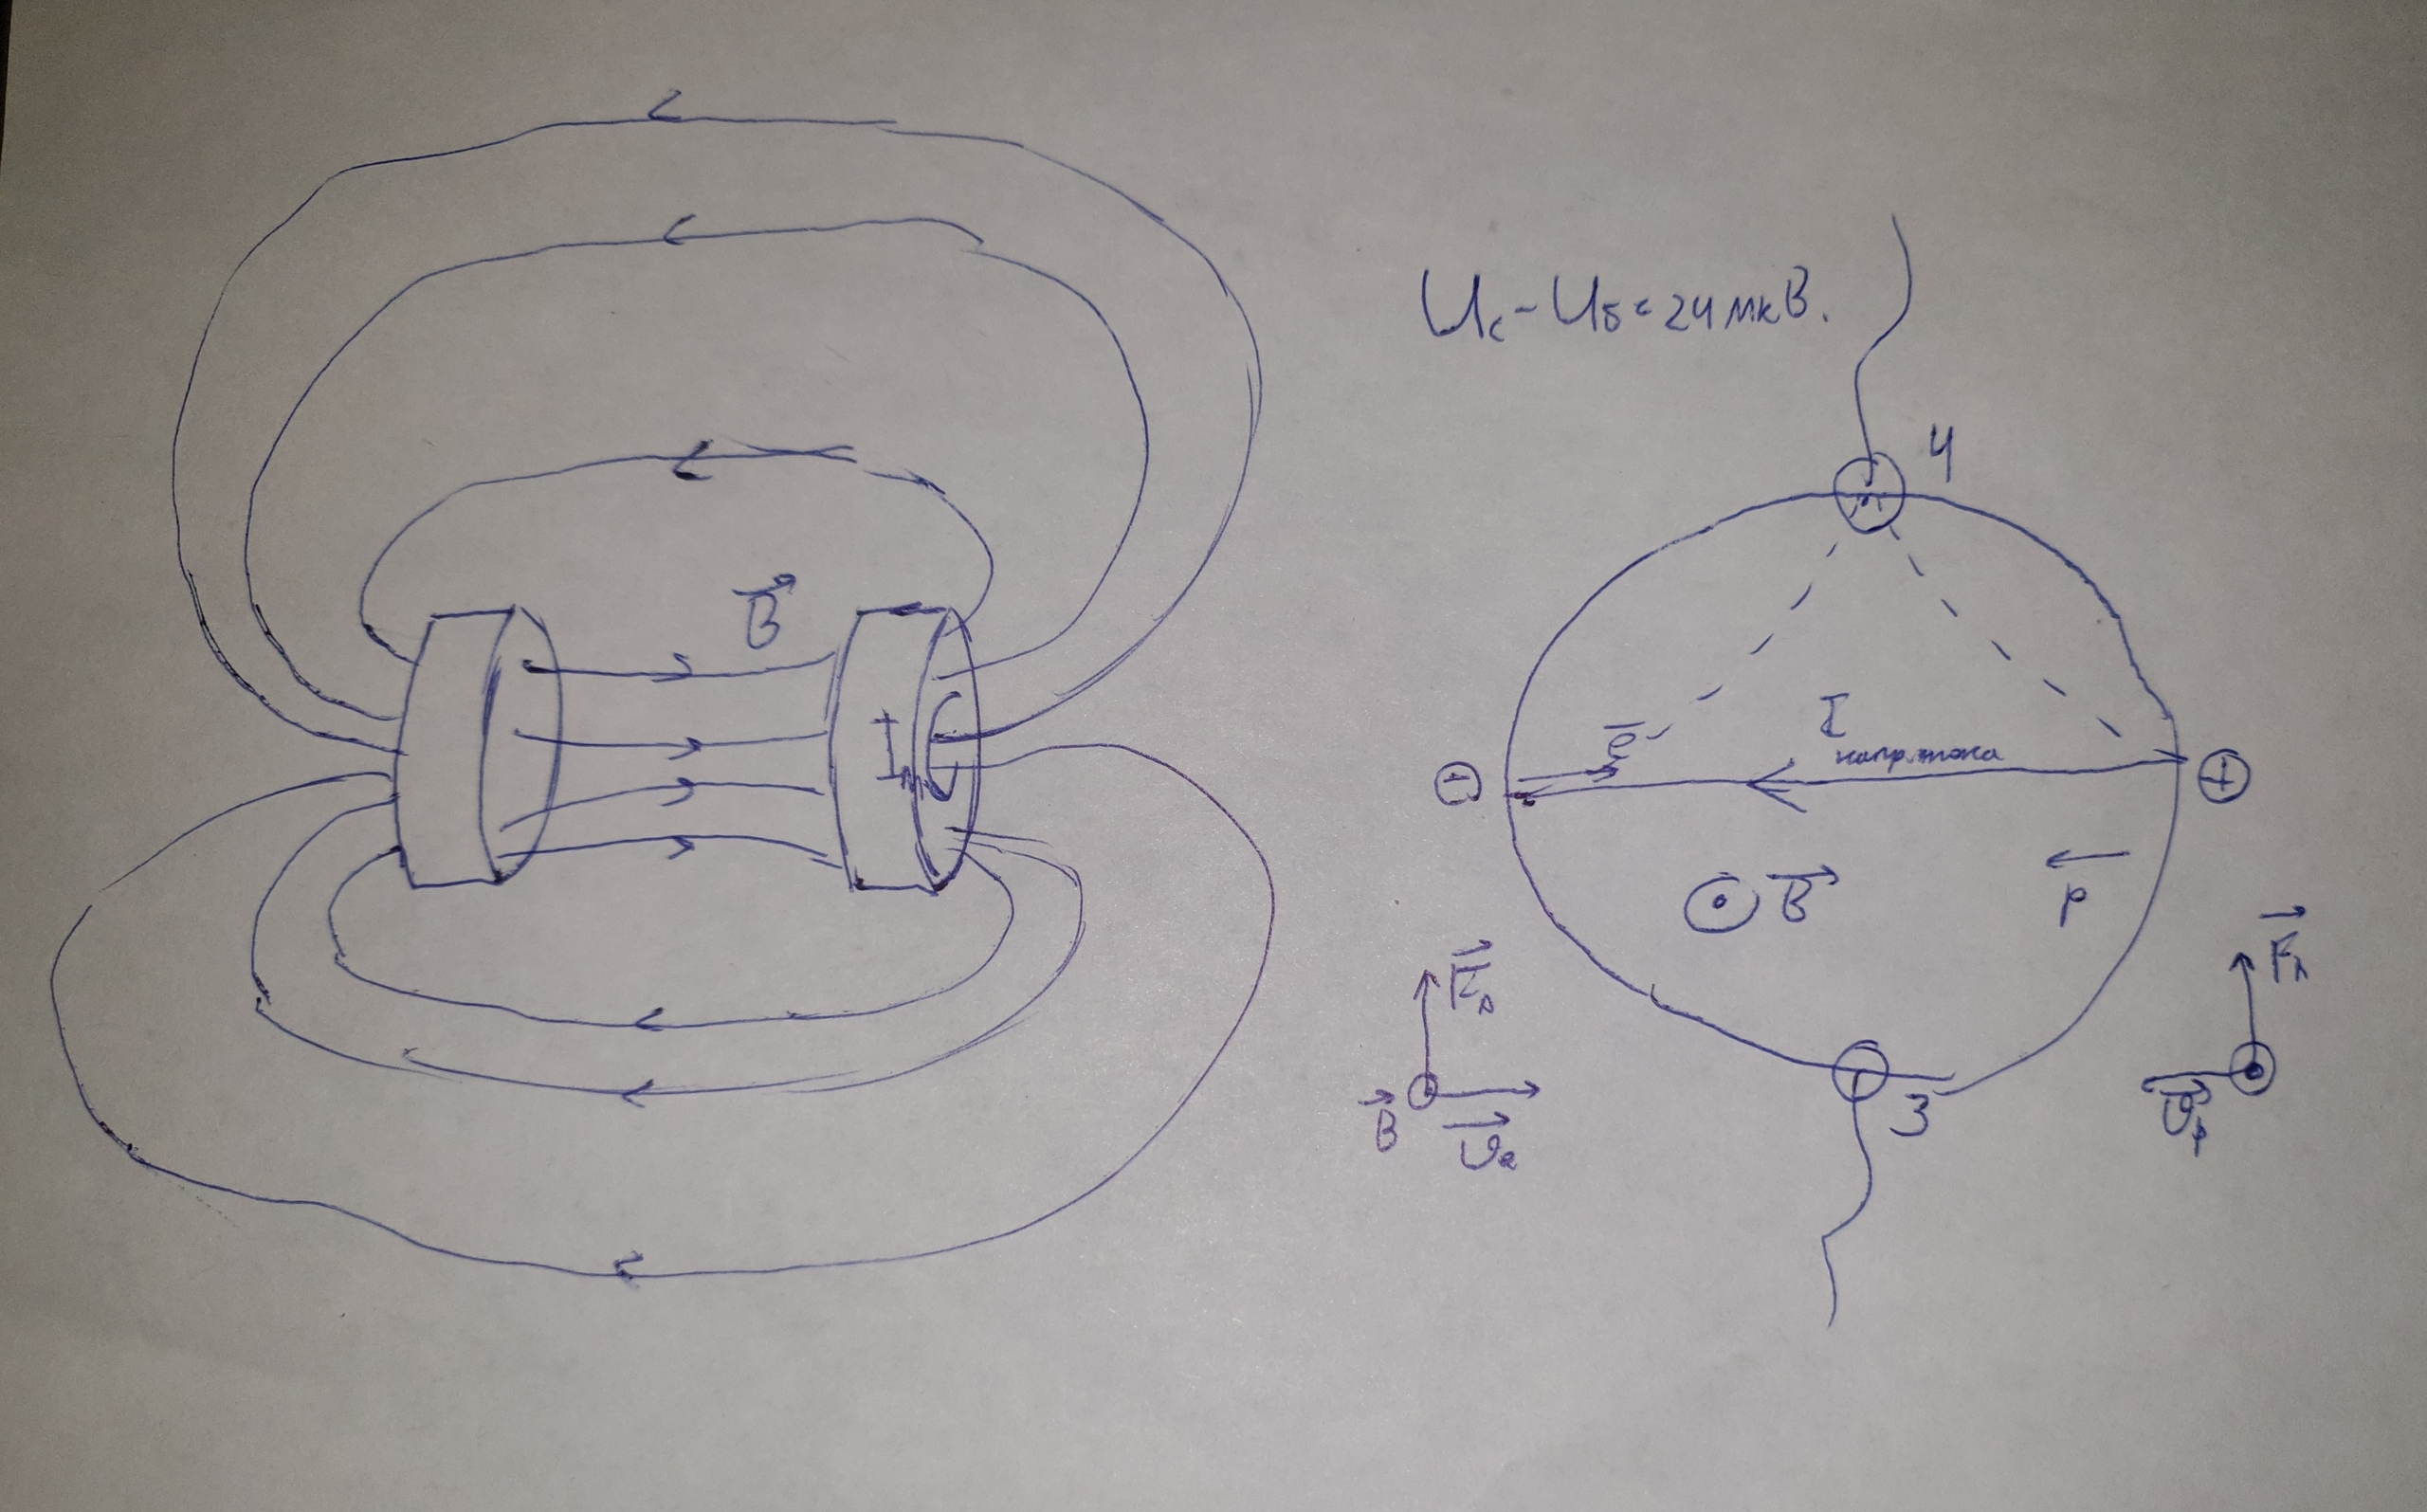
\includegraphics[width=0.8\textwidth]{prov}
\end{center}
\ECaption{Определение характера проводимости}
\end{figure}

Как видно из рисунка, если найти вектор силы Лоренца, направление тока, а так же знак ЭДС Холла, которое в этом случае положительное, то можно заключить, что в легированном германии преобладает проводимость электронного типа.

\subsection*{Определение удельной проводимости}
При токе через образец в 1 мА было измерено падение напряжения между контактами 3-5, 
\begin{equation}
U_{35} = -1.66\pm0.01 \text{ мВ},
\end{equation}
Таким образом, зная, что $L_{35} = 3.0$ мм, $a = 1.5$ мм, $l = 1.7$ мм, используя формулу (5), вычисляем удельную проводимость:
\begin{equation}
\sigma = -708\pm11 \text{ (Ом*м)}^{-1}.
\end{equation}
\section*{Обработка данных}
\subsection*{Градуировка электромагнита}
Используя формулу $\Phi=BSN$, и зная, что $SN = 72\text{ вит*см}^2$, Можем построить график $B = f(I_M)$, он показан на рис 4.

\begin{figure}[h!]
\begin{center}
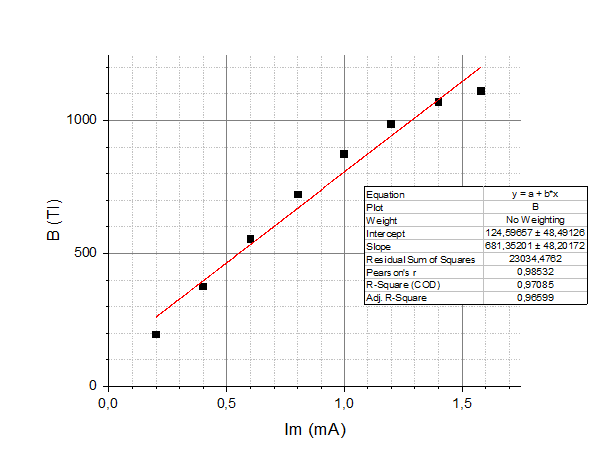
\includegraphics[width=0.8\textwidth]{grbi}
\end{center}
\ECaption{$B = f(I_M)$}
\end{figure}

\subsection*{Определение постоянной Холла}
Построим графики зависимостей $\xi_x=f(B)$, для каждого из токов через образец $(0.3-1.0)$ мА, и линеаризуем каждый график. Для каждого тока получим величину коффициента наклона графика. Все это представлено на рис.5. Отсюда получаем таблицу значений $K(I)$:
\begin{figure}[h!]
\begin{center}
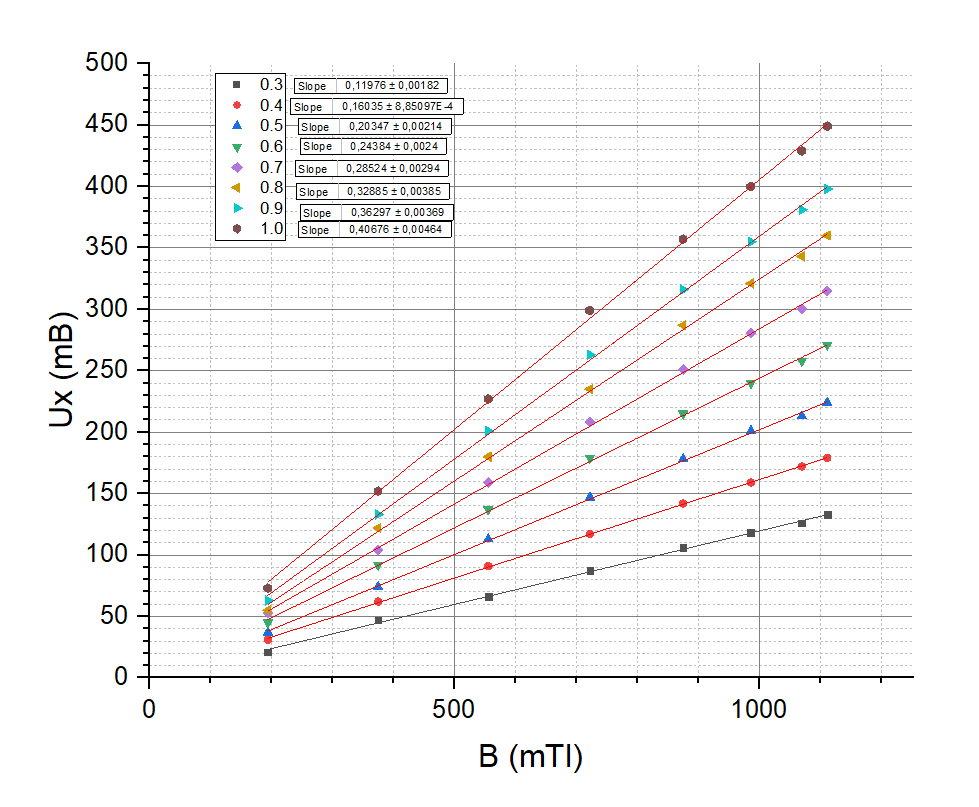
\includegraphics[width=1\textwidth]{grbu}
\end{center}
\ECaption{Очень красивый график}
\end{figure}

\begin{table}[h!]
\begin{center}
\begin{tabular}{|c|l|l|l|l|l|l|l|l|}
\hline
\rowcolor[HTML]{FFFFC7} 
$K$, В/Тл        & 0.12  & 0.16  & 0.203 & 0.244 & 0.285 & 0.33  & 0.363 & 0.407 \\ \hline
$\Delta K$, В/Тл & 0.002 & 0.001 & 0.002 & 0.002 & 0.003 & 0.004 & 0.004 & 0.005 \\ \hline
\rowcolor[HTML]{FFFFC7} 
$I$, мА        & 0.3   & 0.4   & 0.5   & 0.6   & 0.7   & 0.8   & 0.9   & 1     \\ \hline
\end{tabular}
\end{center}
\ECaption{$K(I)$}
\end{table}
Теперь построим график $K=f(I)$, он показан на рис.6.
\begin{figure}[h!]
\begin{center}
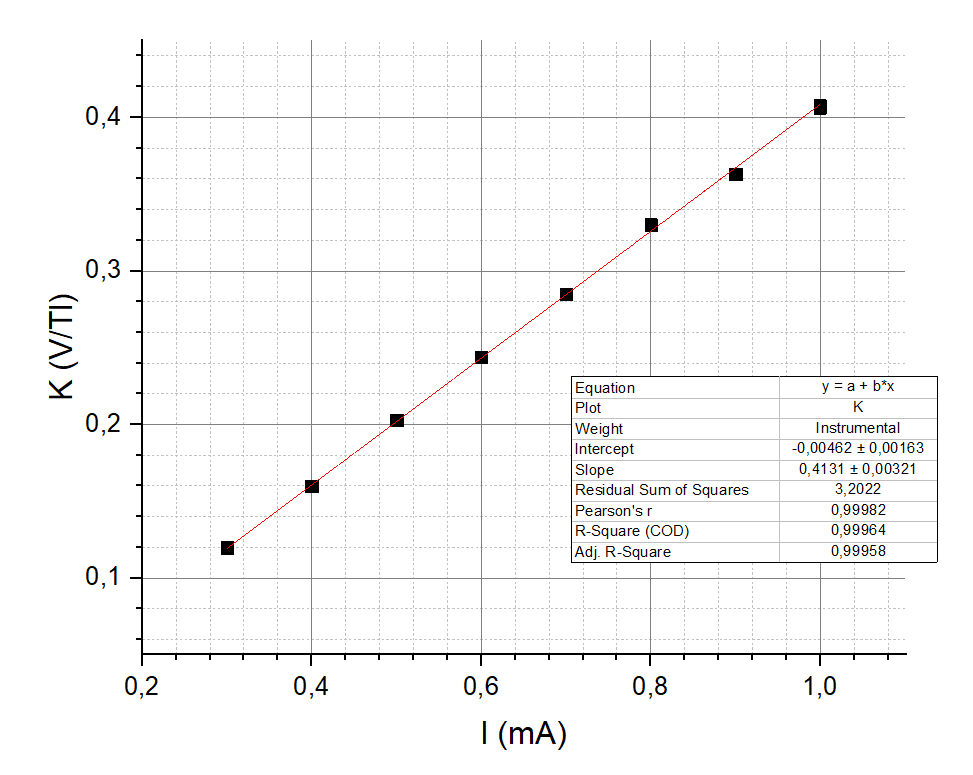
\includegraphics[width=0.9\textwidth]{grki}
\end{center}
\ECaption{$K=f(I)$}
\end{figure}
Из графика видно, что коэффициент наклона этого графика:
\begin{equation}
\alpha=(413\pm3)\text{ B/(Тл*мА)}.
\end{equation}
Используя формулу (3) получаем, что 
\begin{equation}
R_x=-\xi_x\dfrac{a}{IB} = -a\alpha,
\end{equation}
где $a = 1.5$ мм. Окончательные результаты будут представлены в форме таблицы в разделе "Результаты".
\subsection*{Расчет концентрации и подвижности носителей заряда}
С помощью формулы (4) находим концентрацию зарядов:
\begin{equation}
n = \dfrac{1}{eR_x}.
\end{equation}
Далее, зная выражение (1) и проводимость образца, получаем формулу для подвижности:
\begin{equation}
b = \dfrac{\sigma}{en}=\sigma\cdot R_x.
\end{equation}
Погрешности этих значений рассчитываются по известным формулам.
\subsection*{Результаты}
Результаты представлены в виде таблицы.
\begin{table}[h!]
\begin{tabular}{|c|c|c|c|c|}
\hline
\rowcolor[HTML]{FFFFC7} 
$R_x\pm\Delta R_x$, $\frac{\text{м}^3}{\text{Кл}}$ & $n\pm\Delta n$, $\text{м}^{-3}$ & $\sigma\pm\Delta\sigma$, $\text{(Ом*м)}^{-1}$ & $b\pm\Delta b$, $\frac{\text{см}^2}{\text{В*с}}$ \\ \hline
 $-(6.2\pm0.05)\times10^{-4}$        &  $(1.01\pm0.01)\times10^{22}$           &                   $-(708\pm11)$ &  $(4.4\pm 0.1)\times10^2$              \\ \hline
\end{tabular}
\ECaption{Результаты}
\end{table}
Они отлично согласуются со справочными данными и обладают малой ошибкой измерений.
\section*{Вывод}
В соответствии с целью работы измерены подвижность и концентрация носителей заряда с хорошей точностью и степенью согласованности, так же был определен тип этих носителей - это электроны, что соответствует легированному германию. Изучен эффект Холла на лабораторном оборудовании.




\end{document}

